\documentclass{thesis-uestc}


\title{珊瑚-I 入门引导}{aCoral-I Guide Manual}
\author{王彬浩}{Wang BinHao}
\school{信息与软件工程学院}{School of Information and Software Engineering}
\major{电子信息}{Electrical & Information}
\studentnumber{202122090410}
\version{1.3}


% require all the usepackages here
% \usepackage{algorithm2e}
%\usepackage[section]{placeins}
\usepackage{longtable}  %跨页表格
\usepackage{listings}   %代码块
\usepackage{xcolor}     %颜色宏
\usepackage{fontspec}   %字体
\usepackage{caption}    %显示图片和表格的标题
\usepackage{float}      %图片的“H”浮动选项
\usepackage{hyperref}

\hypersetup{hidelinks,
	colorlinks=true,
	allcolors=black,
	pdfstartview=Fit,
	breaklinks=true}


\lstset{
    basicstyle=\small, 
    breaklines,                                 % 自动将长的代码行换行排版
    extendedchars=false,                        % 解决代码跨页时,章节标题,页眉等汉字不显示的问题
    backgroundcolor=\color[rgb]{0.96,0.96,0.96},% 背景颜色
    keywordstyle=\color{blue}\bfseries,         % 关键字颜色
    identifierstyle=\color{black},              % 普通标识符颜色
    commentstyle=\color[rgb]{0,0.6,0},          % 注释颜色
    stringstyle=\color[rgb]{0.58,0,0.82},       % 字符串颜色
    showstringspaces=false,                     % 不显示字符串内的空格
    numbers=left,                               % 显示行号
    captionpos=t,                               % title在上方(在bottom即为b)
    frame=single,                               % 设置代码框形式
    rulecolor=\color[rgb]{0.8,0.8,0.8},         % 设置代码框颜色
    tabsize=4                                   %tab长度为4个空格
}  

\begin{document}

\makecover

% This is a template of mutiple files.
% The folders chapters/ and misc/ have the related files

\begin{revisionhistory}
    \begin{center}
        \setlength\tabcolsep{15pt}
        \begin{tabular}{|c|p{16em}<{\centering}|c|c|}
            \hline  版本号 & 内容 & 日期 & 负责人 \\
            \hline 0.1 & 开始编写,修改latex模板,确定大纲 & 2022.05.15 & 王彬浩 \\
            \hline 1.0 & 第一版aCoral入门引导编写完成 & 2022.06.12 & 王彬浩 \\
            \hline 1.1 & 增加Ubuntu和编译器、dnw工具的下载链接 & 2022.06.14 & 王彬浩 \\
            \hline 1.2 & 修正配置环境时的操作 & 2022.06.14 & 王彬浩 \\
            \hline \Version & 修改3.1 & 2022.07.05 & 王彬浩 \\
            \hline
        \end{tabular}
    \end{center}



\end{revisionhistory}



% table of contents
\thesistableofcontents

% thesis contents
\chapter{概述}

\section{珊瑚(aCoral)简介}

珊瑚(aCoral)是电子科技大学信息与软件工程学院嵌入式智能计算研究团队开发的一款嵌入式实时操作系统,具有开源、高可配、高扩展性的特点。

珊瑚(aCoral)目前拥有单核(aCoral-I)和多核(aCoral-II)两个版本。本仓库中的文档将介绍珊瑚操作系统的单核版本aCoral-I,使用的硬件平台为mini2440。
出于方便的目的,后续将单核版本的珊瑚简称为aCroal。单核版本的珊瑚(aCoral-I)对于主流的开发平台都有支持,像 s3c2440,s3c2410,s3c44b0,lpc2313,lpc2200,stm3210。

aCoral 支持多线程模式,其最小配置生成的代码为 7K 左右,而配置文件系统、轻型 TCP/IP、GUI 后生成的代码仅有 300K 左右。

嵌入式操作操作系统一般都是实时的,但是如何做到强实时是一个很棘手的问题,为强实时计算密集型应用(航空电子、舰载电子„„)提供可靠运行支持
是 aCoral 开发的强力主线。目前 aCoral 提供了强实时内核机制(优先级位图法、优先级天花板协议、差分时间链、最多关中断时间)。与此同时,aCoral 还提供了
强实时调度策略:RM 调度算法,强实时确保策略也正在研究中。

aCoral 会像珊瑚一样成长......

\section{aCoral项目成员}
\subsection{aCoral早期版本项目成员}

\begin{center}
    \setlength\tabcolsep{2pt}
    \begin{longtable}{|p{12em}<{\centering}|p{17em}<{\centering}|}
        \hline  成员姓名 & 主要贡献  \\
        \hline  廖勇 & 项目创建人及总负责人 \\
        \hline  申建晶 & 内核框架设计及实现,GUI 系统 \\
        \hline  闫志强 & 内核线程交互开发及 TCP/IP 协议栈 \\
        \hline  孔帅帅 & 多核支持及中断系统 \\
        \hline  高攀 & 文件系统开发,H.264在ARM11的多核优化 \\
        \hline  陈旭东 & 多核调度、实时性确保、多核实时控制 \\
        \hline  刘晓翔 & 开发环境及驱动模块 \\
        \hline  杨茂林 & 强实时调度算法研究及实现 \\
        \hline  张国梁 & 操作系统移植 \\
        \hline  王小溪 & 系统测试及性能确保、应用程序 \\
        \hline  魏守峰 & 系统测试及性能确保、应用程序 \\
        \hline  任艳伟 & 内核实时性确保 \\
        \hline  程潜 & 内核实时性确保 \\
        \hline  程勇明 & 内核实时性确保 \\
        \hline  汪琳玫 & 功耗管理 \\
        \hline  周强 & 驱动模型设计及自有图形系统开发 \\
        \hline  许斌 & 操作系统配置工具开发 \\
        \hline  袁霞 & 调度算法 \\
        \hline  江维 & 可信调度、功耗管理 \\
        \hline  李波 & 操作系统移植 \\
        \hline  张海斌 & 多核中断支持 \\
        \hline  钟太聪 & 多核调试器 \\
        \hline  彭东脉 & 多核调试器 \\
        \hline  Mugundhan balaji & H.264 多核支持 \\
        \hline  Subhajit Banerjee Purnapatra & 多核调试器 \\
        \hline  孙康 & 内存管理 \\
        \hline  王云飞 & 内存管理 \\
        \hline  郭治姣 & 操作系统移植 \\
        \hline  韩炫 & 操作系统移植 \\
        \hline  文秀春 & 操作系统移植 \\
        \hline  刘坚 & 操作系统移植 \\
        \hline  龚俊儒 & 操作系统移植 \\
        \hline  李天华 & 操作系统移植 \\
        \hline  郭文生 & 多核形式化验证 \\
        \hline  刘洋 & 应用程序 \\
        \hline  熊光泽 & 技术指导 \\
        \hline  桑楠 & 技术指导 \\
        \hline  雷航 & 技术指导 \\
        \hline  罗蕾 & 技术指导 \\
        \hline  李允 & 技术指导 \\
        \hline  陈丽蓉 & 技术指导 \\
        \hline
    \end{longtable}
\end{center}

\subsection{aCoral-I 项目成员}
\begin{center}
    \setlength\tabcolsep{2pt}
    \begin{tabular}{|p{12em}<{\centering}|p{17em}<{\centering}|}
        \hline  成员姓名 & 主要贡献 \\
        \hline  杨茂林 & 项目负责人\\
        \hline  王彬浩 & 代码重构、文档编写、应用开发\\
        \hline
    \end{tabular}
\end{center}
\chapter{aCoral结构}

\section{aCoral系统结构}
aCoral由内核(kernel)和外围模块(Peripheral)两大部分组成。
其中内核又包含中断管理系统、内存管理系统、线程管理系统和线程交互系统;
外围模块包括驱动管理、图形用户界面(GUI)、文件系统和网络模块(Net)。
如图2-1所示。

\begin{figure}[H]
	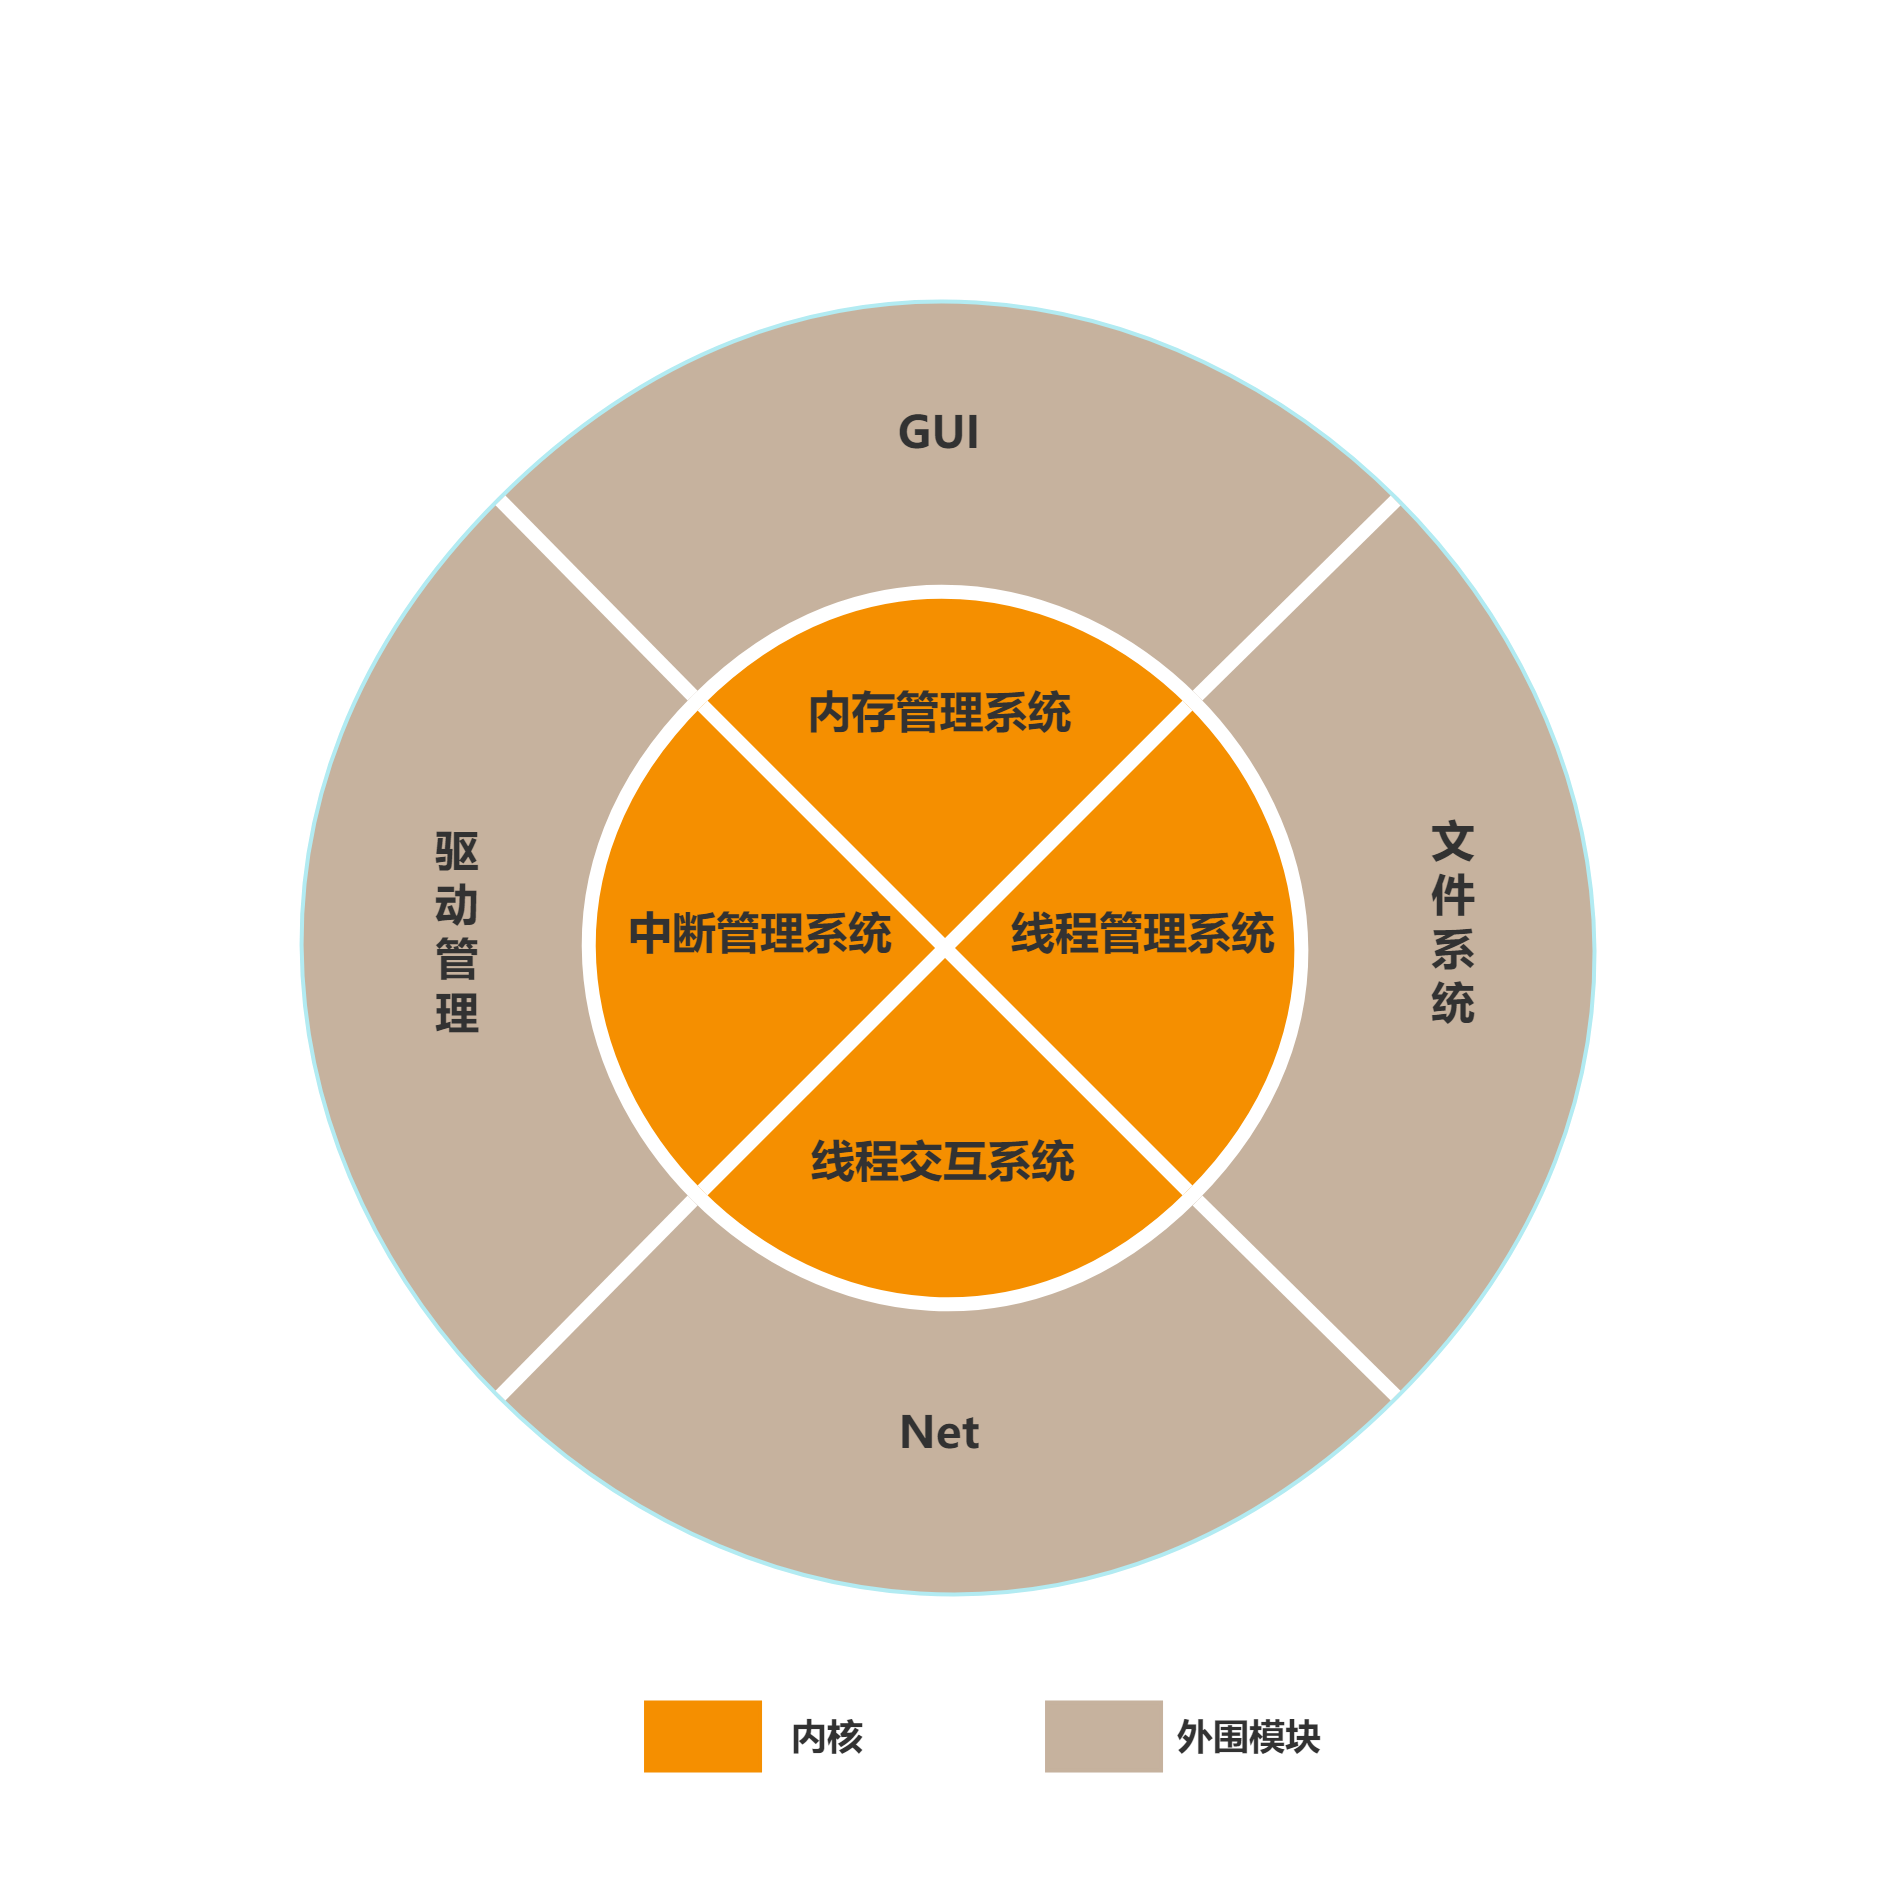
\includegraphics[width=400pt]{aCoral系统结构.png}
	\caption{aCoral系统结构}
	\label{pica}
\end{figure}

内核当中,中断管理系统负责响应并处理处理来自外部和内部的所有中断(异常),例如时钟中断、按键中断等;
内存管理系统负责对mini2440上的SDRAM内存进行管理,包括内存的分配、回收算法的实现;
线程管理系统包括线程调度机制和线程调度策略两个部分,负责创建、挂起、杀死线程等操作以及按照何种策略来调度线程;
线程交互系统包括互斥量、信号量、邮箱、消息队列等线程间交互机制。

\section{aCoral文件结构}

aCoral 的一大特点是可配置性,这就要求好的系统文件结构。aCoral内核主要由7个文件夹组成:

(1)kernel,内核文件夹.该文件夹下又有两个文件夹:

	\chinesespace i. include:内核模块的头文件目录

	\chinesespace ii. src:内核模块的源码目录
 
(2)hal(Hardware Abstract Layer),硬件抽象层文件夹。这里存放各种开发板硬件相关的底层代码。

(3)include,aCoral一些重要配置头文件。

(4)driver,驱动文件夹。此文件夹存放系统的驱动程序:

	\chinesespace i. src,这里存放平台无关驱动模型实现,比如驱动模型,sd 卡驱动模型。

	\chinesespace ii. include, 这里存放平台无关驱动模型的头文件,比如 screen 设备的信息结构,触摸屏设备的信息结构。

	\chinesespace iii. 开发板相关驱动文件夹,s3c2440,s3c2410,每个文件夹下又各自包含include,src 文件夹。

(5)plugin,项目扩展插件目录,比如文件系统,图形系统,TCP/IP 协议栈等等。

	\chinesespace i. src,扩展插件的公共源码。

	\chinesespace ii. include ,扩展插件的公共头文件。

	\chinesespace iii. 具体的扩展插件文件夹。

(6)lib,库目录。

	\chinesespace i. src,源码目录。

	\chinesespace ii. include,头文件

(7)user,用户程序目录。

	\chinesespace i. src,源码目录。user.c 中的 user\_main 是用户程序的入口函数,大家可以在这个函数里添加自己的应用。

	\chinesespace ii. include,头文件

(8)test,测试文件目录。主用用于内部测试。

	\chinesespace i. src,源码目录。

	\chinesespace ii. include,头文件

除了这些文件夹以外,aCoral根目录下还有一些重要的文件,Makefile、dnw.c、.config(menuconfig自动生成)……
这些文件都有十分重要的作用,可以有空自行学习。另外那些acoral打头的文件则是在编译过程中自动生成的一些辅助文件,有助于开发人员debug和开发应用。

\chapter{使用介绍}

在这一章中,手册使用的操作系统为Ubuntu 18.04.5 LTS,编译交叉工具链为arm-2010q1。其它版本的操作系统和编译器可以自行测试。
点击 \href{https://github.com/spg-one/aCoral1-Tools}{\underline{工具链接}} 下载所需工具。

\section{配置编译环境}

(1)第一步,修改编译所需的编译器。修改aCoral根目录下的Makefile文件中的交叉编译路径CROSS\_COMPILE 为
\begin{lstlisting}
 xxx/arm-2010q1/bin/arm-none-eabi-
\end{lstlisting}

其中“xxx”为交叉编译链文件所在路径。

(2)第二步,编译。进入aCoral根目录,在终端输入
\begin{lstlisting}
 make
\end{lstlisting}

如果出现"no such file or directory"的错误,则是因为32位编译器不能在64位系统中运行,需要安装32位库。
在终端中输入
\begin{lstlisting}
 apt-get install lib32ncurses5 lib32z1
\end{lstlisting}

安装完成后,再次输入make即可。

等待编译完成之后,就会得到我们要下载的aCoral镜像文件acoral.bin以及一些辅助文件。




\section{aCoral内核下载}

在得到acoral.bin镜像文件后,我们就可以将其下载到开发板上了。
理论上我们可以直接把acoral.bin烧写到开发板的nor flash或者nand flash上启动,aCoral可以自我引导,即将自己复制到sdram内存中执行。
但是这有一个问题,烧写到nor flash或者nand flash的速度是很慢的,如果我们每次在修改aCoral的源码后,
直接烧写到开发上进行调试,就会浪费大量时间在等待烧写完成上。

对于这个问题,我们有一种解决方案,就是在nor flash或者nand flash中烧写一个bootloader,每次修改源码编译得到新镜像后,
使用bootloader,将新编译得到的内核镜像直接复制到sdram中执行,这样就可以节省很多时间。
本手册中,bootloader我们使用友善之臂开发的supervivi。关于supervivi如何烧写进flash,请自行在网上查找资料。
这里我们默认已经在nor flash中烧写好了supervivi。接下来就可以正式开始下载aCoral。

(1)第一步,接线。依次从左到右为USB下载线、串口线、电源线,如图\ref{接线示意图}。
\begin{figure}[H]
	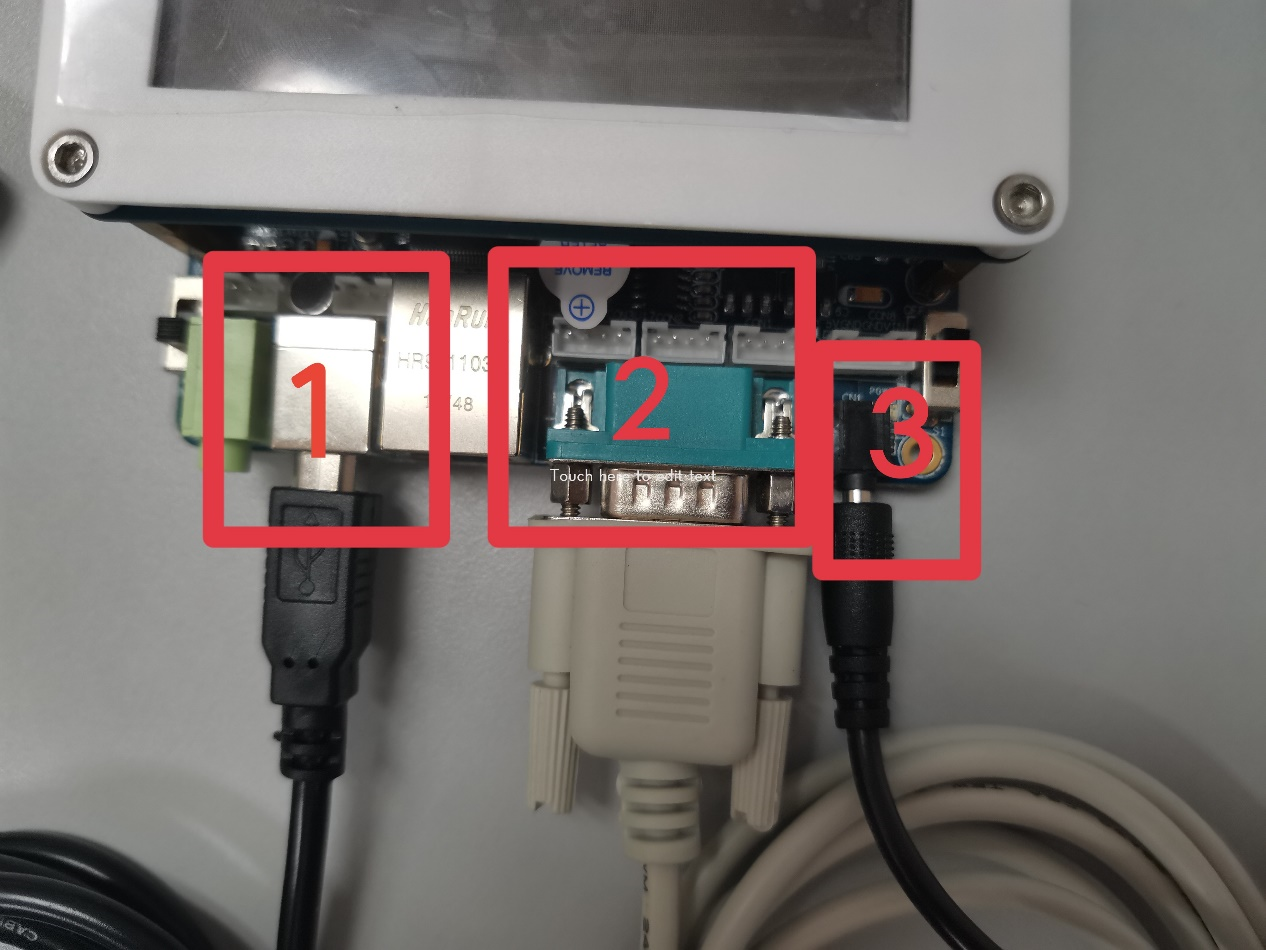
\includegraphics[width=0.9\textwidth]{接线示意图.png}
	\caption{接线示意图}
	\label{接线示意图}
\end{figure}

大家电脑上肯定没有串口了,所以需要接一个USB转串口线(PL2303芯片)。驱动安装
参考 \href{https://blog.csdn.net/qq_34562093/article/details/75059251}{\underline{ubuntu安装USB转串口驱动}}

(2)第二步,安装mimicom串口工具,并能够正确识别插上的USB转串口。具体自行查阅资料。成功连接串口界面如图\ref{minicom初始}:
\begin{figure}[H]
	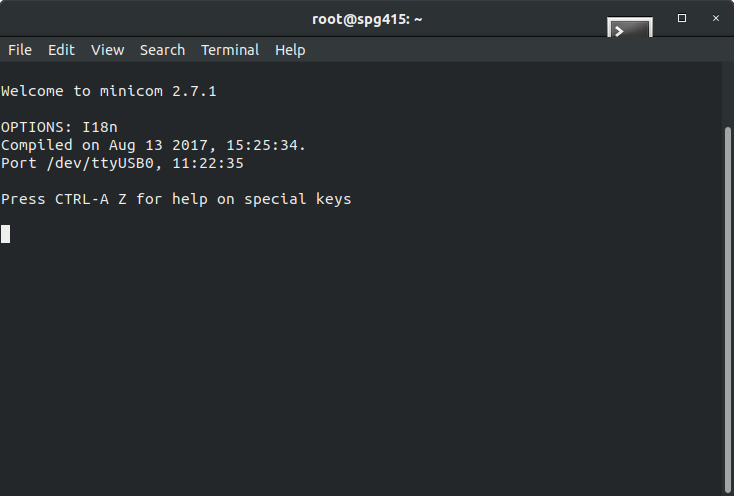
\includegraphics[width=0.9\textwidth]{minicom初始.png}
	\caption{minicom初始界面}
	\label{minicom初始}
\end{figure}

(3)第三步,将开发板左下角的开关向下拨到nor,如图\ref{nor开关}所示。
\begin{figure}[H]
	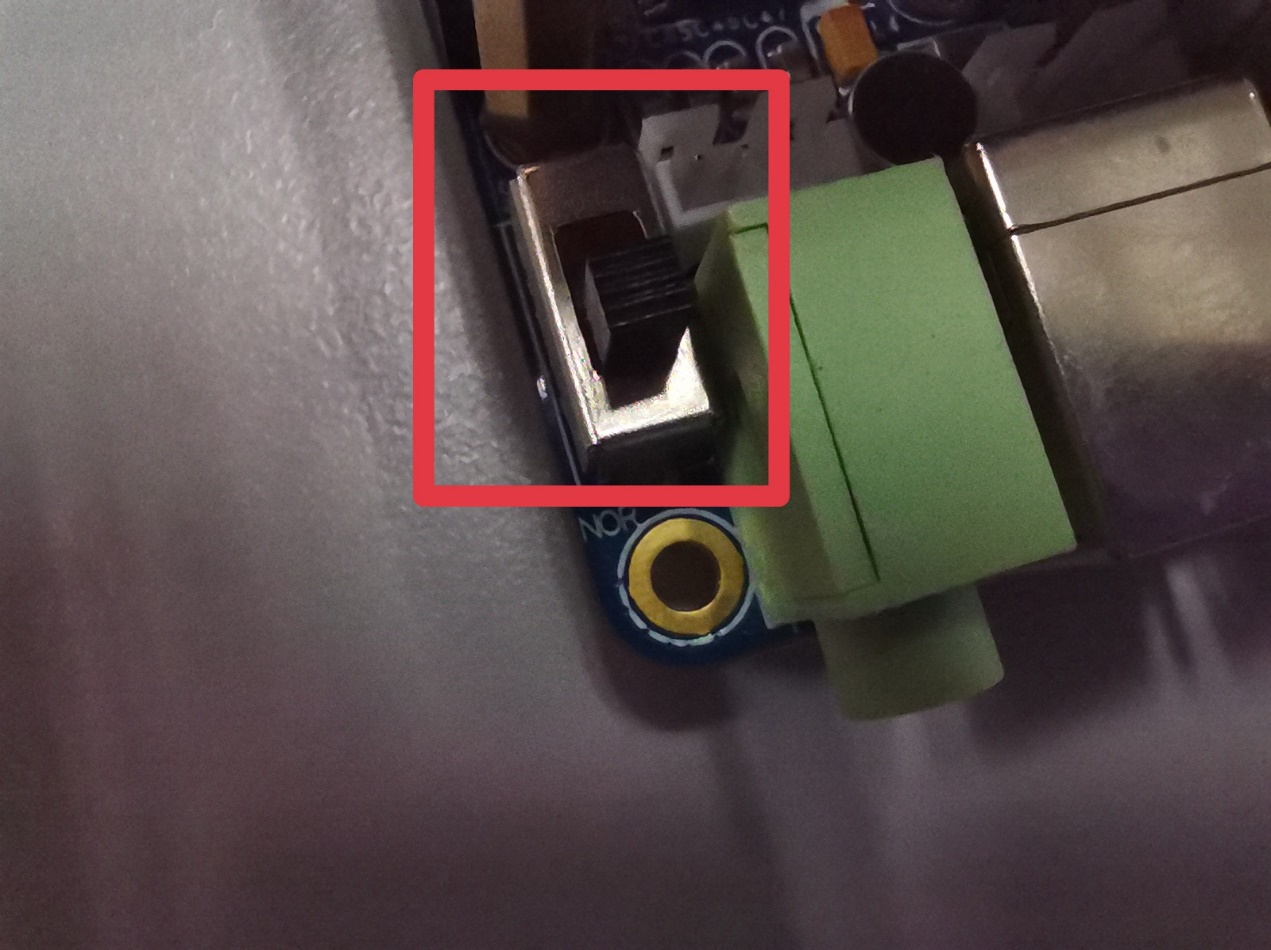
\includegraphics[width=0.9\textwidth]{nor开关.png}
	\caption{nor开关}
	\label{nor开关}
\end{figure}

(4)第四步,编译之前下载的工具目录下的dnw.c文件。这里我们已经提前编译好了dnw,直接使用即可。dnw就是USB下载线的驱动。

(5)运行minicom,打开mini2440的电源,你将看到如图\ref{supervivi界面}所示界面:
\begin{figure}[H]
	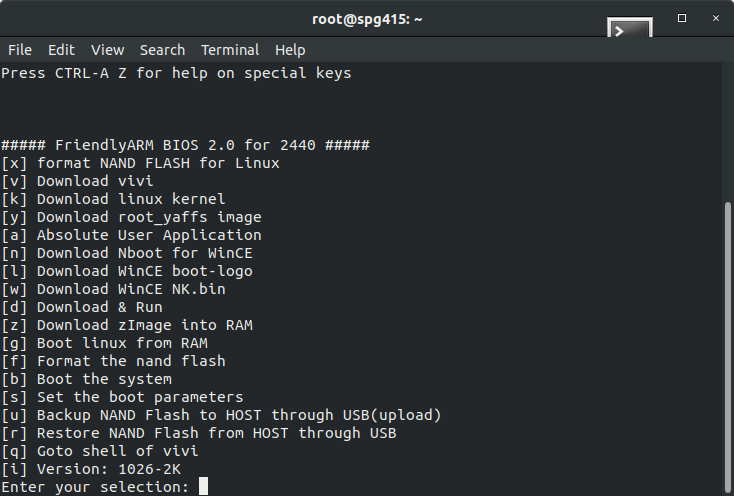
\includegraphics[width=0.9\textwidth]{supervivi界面.png}
	\caption{supervivi界面}
	\label{supervivi界面}
\end{figure}

输入d,看到如图\ref{等待USB下载}所示界面:
\begin{figure}[H]
	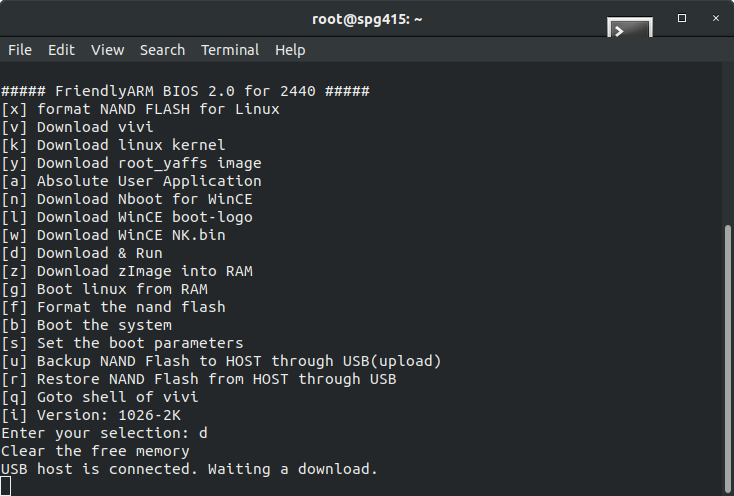
\includegraphics[width=0.9\textwidth]{等待USB下载.png}
	\caption{等待USB下载}
	\label{等待USB下载}
\end{figure}

运行dnw,下载acoral.bin,如图\ref{dnw下载}:
\begin{figure}[H]
	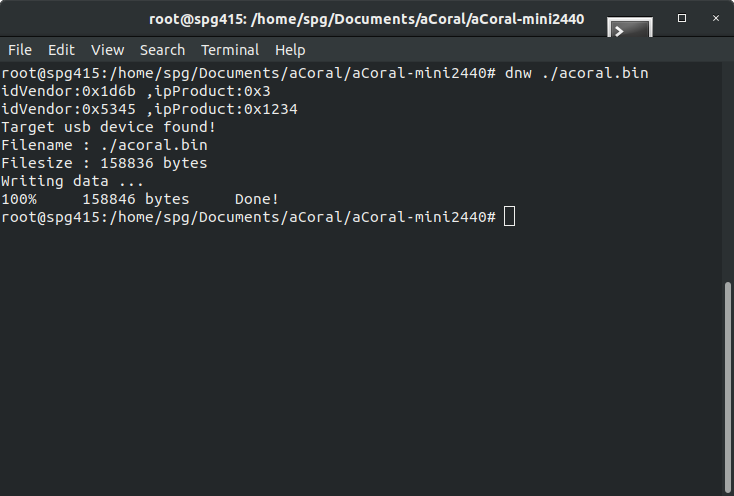
\includegraphics[width=0.9\textwidth]{dnw下载.png}
	\caption{dnw下载}
	\label{dnw下载}
\end{figure}

如果一切顺利,你将在minicom看到如图\ref{aCoral shell}所示的界面:
\begin{figure}[H]
	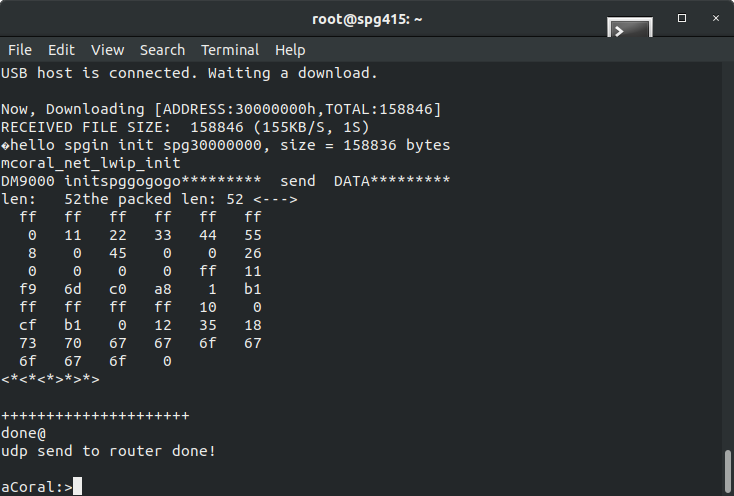
\includegraphics[width=0.9\textwidth]{aCoral shell.png}
	\caption{aCoral shell}
	\label{aCoral shell}
\end{figure}

大家可以在中输入help命令,看看aCoral现在支持的指令,如图\ref{help命令}所示:
\begin{figure}[H]
	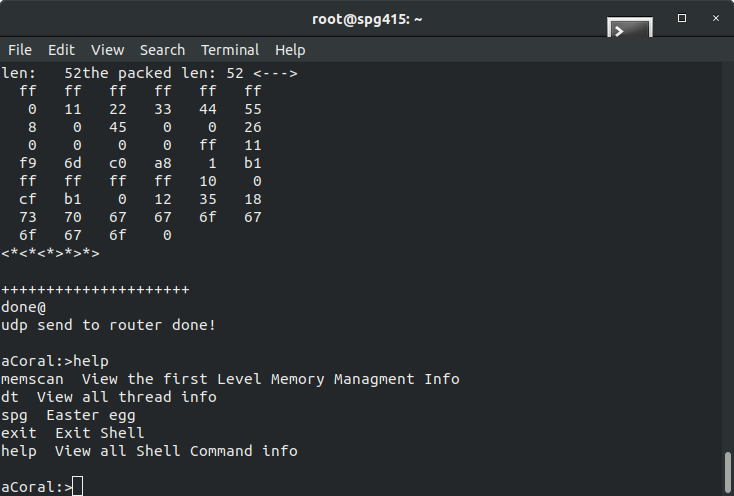
\includegraphics[width=0.9\textwidth]{help命令.png}
	\caption{help命令}
	\label{help命令}
\end{figure}

至此,aCoral的下载完成,之后如果又重新编译了新的镜像,都可以按照这个步骤来。
需要注意的是,这种使用bootloader直接往sdram下载的镜像,关机之后没了,需要重新下载。
\chapter{相关资料}
根目录下的Appendix文件夹内放有在学习aCoral过程中会用到的一些第三方文档。 



\end{document}
